\documentclass[twocolumn]{jsarticle}
\usepackage[dvipdfmx]{graphicx}
\usepackage{here}
\usepackage{url}
\usepackage{okumacro}
\usepackage[%
 dvipdfmx,% 欧文ではコメントアウトする
 setpagesize=false,%
 bookmarks=true,%
 bookmarksdepth=tocdepth,%
 bookmarksnumbered=true,%
 colorlinks=false,%
 pdftitle={},%
 pdfsubject={},%
 pdfauthor={},%
 pdfkeywords={}%
]{hyperref}


%二段組にするやつの設定
\setlength{\columnsep}{2zw}
\setlength{\columnseprule}{0.4pt}

%

%タイトル
\title{令和5年 5学年保健体育レポート}%タイトル
\author{本間 三暉(電子制御工学科 5学年 35番)}%名前
\date{}

\begin{document}
\twocolumn[%
  \centering
  \maketitle
]

\section{暑熱順化}
\subsection{暑熱順化とは}
暑熱順化とは体が暑さに慣れることである.暑い日が続くと,体は次第に暑さに慣れて暑さに強くなる.


\subsection{暑熱順化による変化}
人は運動や仕事などで体を動かすと体内で熱が作られて体温が上昇する.
体温が上がったときは発汗による気化熱や,心拍数の上昇や皮膚血管拡張によって体の表面から空気中に熱を逃がす熱放散で体温を調節している.
この体温の調節がうまくできなくなると体の中に熱が溜まって体温が上昇し熱中症が引き起こされる.

暑熱順化が進むと,発汗量や皮膚血流量が増加し,発汗による気化熱や体の表面から熱を逃がす熱放散がしやすくなる.
暑熱順化による体の変化についてまとめた画像を\ref{kill1} に示す.

\begin{figure}[H]
  \centering
  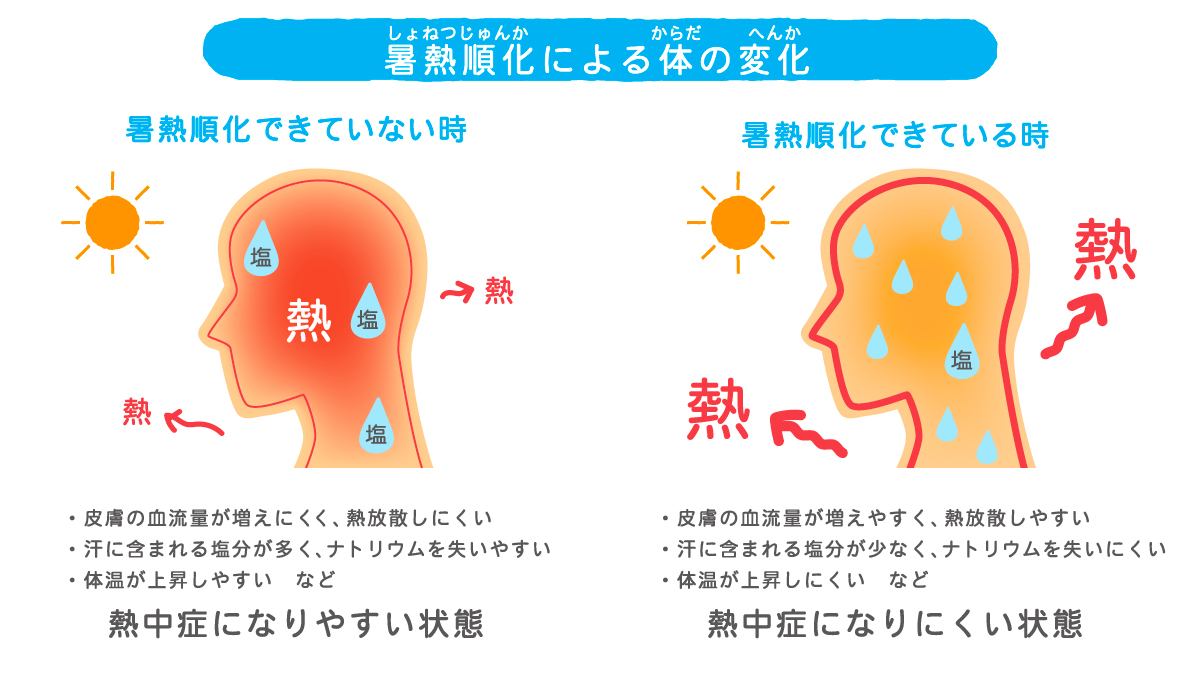
\includegraphics[width=6cm]{kill_1.jpg}
  \caption{暑熱順化による体の変化}
  \label{kill1}
\end{figure}

\subsection{暑熱順化に有効な対策}
体を暑さに慣れさせることが大切であるため,実際に気温が上がり熱中症の危険が高まる前に無理のない範囲で汗をかくことが大切である.

\section{SDGs 達成に向けてあなたのクラスの今現在の達成率}
  私のクラスのSDGs達成率は70\%と考える.
  理由は大きく分けて2つあるが,1つ目は私のクラスのタブレット普及率がかなり高いからである.
  これにより普段の授業などで使う紙の量が他の学年や学校に比べかなり少ないはずである.

  2つ目は移動授業の際は気がついたら電気やエアコンの電源を落としているからである.
  完全に落としているとは言えない場合もあるためそのあたりも加味して70\%と考えている.


\section{授業の自己評価}
まず,令和五年の保健体育のシラバスを参照すると,技能40,レポート40,その他20となっている.

クラス平均が7割となるので,これを基準に考える.

技能の部分であるが,特出して悪い記録を残しているわけではないので全体的に平均より少し上程度の成績ではないかと考える.よって,40点の7割より少し上と考えると,およそ30点が妥当だと考える.

私のクラスは出せばいいと考える人も多くいるので,そういう人は適当な出来のレポートを出す.
そういうのを含めて7割なので,相対的にレポートの内容がしっかりしていて,形式にもしっかり従っている私のレポートは35点であると考える.

最後にその他の点数であるが,これに関して何を参照するのかはわからないが,態度や加点用の場所だとすると,卓球のリーダーをしていることや,やむを得ない事情以外で休んでいないことを考えると満点ではないかと考えられる.

以上の考察から,私の五年前期の保健体育の点数は85点だと考えられる.

\section{授業に対しての要望}

\section*{参考文献}
\begin{enumerate}
  \item \href{https://kawakita.or.jp/aisafetynet/aistation/news/「温熱順化」をご存知ですか?/}{「暑熱順化」をご存知ですか? | あいセーフティネット}
  \item \href{https://www.netsuzero.jp/learning/le15}{暑熱順化 | 熱中症ゼロへ - 日本気象協会推進}
  \item \href{https://syllabus.kosen-k.go.jp/Pages/PublicSyllabus?school_id=16&department_id=14&subject_id=0102&year=2018&lang=ja}{長岡高専シラバス}
\end{enumerate}
\end{document}